\documentclass[11pt, letterpaper]{article}
\usepackage[T1]{fontenc}
\usepackage[spanish]{babel}
\usepackage[margin=2.5cm]{geometry}
\usepackage{setspace}
\usepackage{charter}
\usepackage{float}
\onehalfspacing % Interlineado de 1.5
\setlength{\parskip}{1em} % Espaciado entre párrafos

% Paquetes matemáticos y gráficos (útiles si tu ensayo lo requiere)
\usepackage{amsmath}
\usepackage{graphicx}
\usepackage{hyperref}

% Cambio de la cardinalida para la secciones 
\renewcommand{\thesection}{\Roman{section}}
\renewcommand{\thesubsection}{\alph{subsection}}


% 1. Cargar el paquete de Lua
\usepackage{luacode} 

% 2. Definir la lógica del contador en Lua
\begin{luacode*}
local char_count = 0

function count_chars(head)
    for n in node.traverse(head) do
        if n.id == node.id("glyph") then
            char_count = char_count + 1
        end
    end
    return head
end

function start_counting()
    luatexbase.add_to_callback("pre_linebreak_filter", count_chars, "contador")
end

function stop_counting()
    luatexbase.remove_from_callback("pre_linebreak_filter", "contador")
end

function print_count()
    tex.print(char_count)
end
\end{luacode*}

% 3. Crear los comandos de LaTeX para invocar las funciones de Lua
\newcommand{\iniciarconteo}{\directlua{start_counting()}}
\newcommand{\detenerconteo}{\directlua{stop_counting()}}
\newcommand{\totalcaracteres}{\directlua{print_count()}}







% Datos del ensayo
\title{\textbf{Lo que entendí sobre: "Computational Information Design"}}
\author{@Char[50] \textit{Carlos Mendoza}}
\date{\today}


\begin{document}
\begin{titlepage} 
    \centering
    \vspace*{2cm}
    {\LARGE \textbf{Ensayo sobre los capítulos 1-5: \textit{Computational Information Design}}} \\[2cm]
    {\large 2243030286-LTSI-DCCD} \\[1cm]
    {\large Universidad Autónoma Metropolitana Unidad Cuajimalpa} \\
    {\large Laboratorio Temático II} \\[2cm]
\end{titlepage}
\newpage

% 2. Cuerpo del Ensayo
\maketitle % Muestra el título si omites la portada
\tableofcontents

\newpage
\section{Introducción}
A lo largo de las siguientes páginas quedarán plasmadas mis impresiones acerca de los primeros capitulos del libro \textbf{"Diseño de inforamación Computacional"} \textit{(traducción literal del inglés)} del autor \textbf{Benjamin Frey}. Con el fín de ilustrar al lector con mi perspectiva, incluiré múltiples puntos que considero de gran interés resaltar; puesto que permiten dar con el motivo fundamental tras el porqué, todo esto me resulta inmensamente fascinante.   

\iniciarconteo
\newpage
\section{Sobre el capítulo 1}
Durante este primer paso en el camino de la \textbf{comprensión de datos}, dicho nos brinda un breve pero conciso vistazo sobre una perspectiva general sobre la que, tristemente, se posa una problemática demasiado generalizada a lo largo y ancho del mundo. Típicamente, cada uno de los campos referentes al uso o adquisición de datos, como lo pueden ser la minería de datos, la ciencia computacional o la estadística, suelen resolver de forma extremadamente aislada una ínfima parte de un problema mucho mayor, problema que precisamente el Diseño de Información Computacional guarda entre sus manos. Además de éste hecho, el autor nos hace mención de lo increíblemente extraño y dificil que suele ser que una persona sea suficientemente versada en varios de estos campos a la vez, de tal manera que pueda aprovechar adecuadamente los métodos que sólo ciertas disciplinas pueden proveer; y así, enfrentar cada uno de los pasos siguientes de forma eficiente. 

    \subsection{Los 7 \textit{pasos} del C.I.D.}
    Además de lo mencionado, el autor nos hace notar 7 \textbf{"pasos"} (no en el sentido meramente secuencial, sino más bien como puntos necesarios) que deben recorrerse al menos una vez para lograr que cierto conjunto de datos, pueda convertirse en información clara, atractiva e interactiva. Tales pasos son: 
    \begin{itemize}
        \item Adquirir: Es el hecho de recopilar o utilizar un conjunto de datos ya existente.
        \item Analizar: Escencialmente consiste en tomar dicho conjunto y transformarlo en una estructura más accesible. 
        \item Filtrar: Toma sólo ciertos datos del conjunto completo para representarlos.  
        \item Minar: Aplica cierto metódo matemático o estadístico para evaluar los datos filtrados.
        \item Representar: Busca realizar un boceto simple sobre cómo representar la información obtenida.
        \item Refinar: Trabaja sobre el boceto para llegar una representación mucho más atractiva. 
        \item Interactuar: Añade la capacidad de interacción para que un posible usuario pueda cambiar ciertos parámetros. 
    \end{itemize}
    \textit{(Estos conceptos se definen de forma un tanto escueta, puesto que más adelante tomarán mucho más peso en la narrativa)}

    \newpage
    Todos estos pasos forman parte de un proceso realmente complejo y profundo sobre el manejo y transformación de datos, con la finalidad de obtener información debidamente represetada. La palabra \textbf{"debidamente"} se utiliza, en el sentido de enunciar que la informacion obtenida y su respectiva representación no se remite a un único campo, sino que se vuelve una mezcla de múltiples disciplinas y sus respectivos métodos. Tal cómo se muestra a continuación.    

    \begin{figure}[H]
        \centering
        \renewcommand{\figurename}{Imagen}
        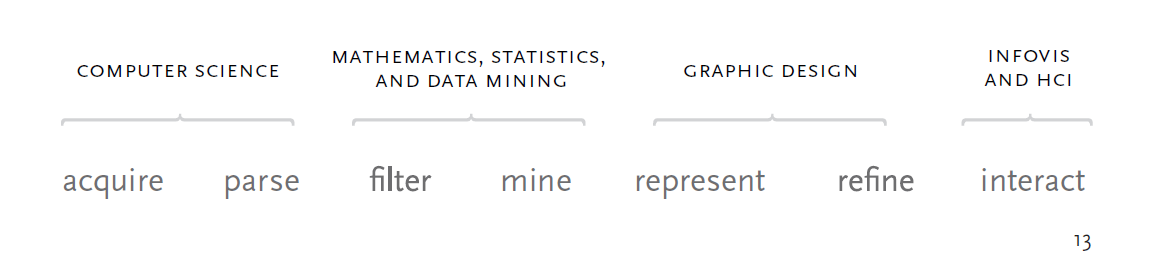
\includegraphics[scale=0.45]{../images/campos.png} 
        \caption{Definición de los campos involucrados en cada paso}
        \label{fig_camp}
    \end{figure} 

    Durante los penúltimos párrafos del capítulo nos habla sobre importancia del uso de herramientas; dando a enteder que éstas deben potencializar nuestras capacidades para llevar a cabo una labor, más allá del hecho de ahorrarnos cierto trabajo y esfuerzo en ello (algo que menciona por el simple hecho de haber co-desarrollado un IDE basado en Java, centrado en el tema del libro). Al final del todo, toca someramente el tema del \textbf{Dominio} como algo que tiende a ser cambiante, así como la particularidad de cada problema. Sin embargo, es innegable mencionar que inclusive algo tan complejo sigue atendiendo a ciertos principios fundamentales. 


\detenerconteo   
\textbf{Total de caracteres en el cuerpo del documento:} \totalcaracteres

\newpage
\section{Sobre el capítulo 2}
Este es el cuerpo principal de tu ensayo. Puedes citar fuentes utilizando el entorno estándar para referenciar ideas.

\newpage
\section{Sobre el capítulo 3}
Resume tus ideas principales y cierra el ensayo con una reflexión final contundente.

\newpage
\section{Sobre el capítulo 4}

\newpage
\section{Sobre el capítulo 5}

\newpage
\section{Conclusiones}



% 3. Referencias
\newpage
% Use BibTeX bibliography; include all entries if none are cited
\bibliographystyle{plain}
\bibliography{references}
\nocite{*}
\end{document}
